\subsection{RQ2b: a training-free fix at the layer the tools point to}
\label{sec:readout}
The find results suggest a fix that needs neither training nor data: at layer~9 the last token still carries the true
sentiment, and the name's information has not reached it yet (Sec.~\ref{sec:find}). We read this state out and add it
back at the end (Sec.~\ref{sec:setup}). In effect this is an early exit at layer~9, the mechanism Halawi et
al.~\cite{halawi2024overthinking} used to undo late-layer failures with false demonstrations; our question is whether
the layer chosen by the find tools is the right place for it.

\textbf{First test.} With $l^*=9$ ($\alpha =$ \pSixAlphaLNineFullFT), the read-out removes \pSixRemovedLNineFullFT{} of
the gap while acc(\textit{none}) drops by only \pSixDropLNineFullFT. A random direction of the same norm at the same
$\alpha$, however, also removed \pSixRemovedRandomFullFT{}; we had required it to remove less than half as much, which
held only in seed 2. Post-hoc, the random vector achieves this by damaging the model: it lowers acc(\textit{none}) by
\pSixDropRandomFullFT.

\textbf{Controlled follow-up.} We therefore registered four controls before running them (Table~\ref{tab:readout},
Fig.~\ref{fig:readout}). With the same total added signal for every $l^*$, layer~9 removes \pSixBEqLNineRemovedFullFT,
more than layers 10 (\pSixBEqLTenRemovedFullFT) and 11 (\pSixBEqLElevenRemovedFullFT), while layers 3 and 6 remove almost
nothing (\pSixBEqLThreeRemovedFullFT; \pSixBEqLSixRemovedFullFT). Given its own $\alpha$ under the same accuracy limit
($\alpha =$ \pSixBRandomAlphaFullFT), the random vector removes only \pSixBRandomRemovedFullFT. Choosing $\alpha$ without
any knowledge of the cue, as the largest value that keeps the accuracy drop on name-free development reviews within
0.02, gives $\alpha =$ \pSixBCueFreeAlphaFullFT{} and removes \pSixBCueFreeRemovedFullFT. Most of the effect comes from the
component of the signal along the unembedding's sentiment direction (\pSixBParRemovedFullFT); the remaining component
removes \pSixBPerpRemovedFullFT, which may reflect sentiment information that this linear projection misses, since it
ignores the final layer norm. The clean twins are barely affected (gap \pSixCleanGapBeforeFullFT{} before and
\pSixCleanGapAfterFullFT{} after the first test).

\begin{table}[t]
\centering
\caption{Training-free read-out fixes on the full fine-tuned shortcut models (seed 0/1/2): fraction of the gap removed
and drop in acc(\textit{none}). The lens row is the post-hoc comparison.}
\label{tab:readout}
\setlength{\tabcolsep}{2.5pt}
\begin{tabular}{lcc}
\toprule
 & Removed & acc(\textit{none}) drop \\
\midrule
Read-out $l^*=9$, first test  & \pSixRemovedLNineFullFT & \pSixDropLNineFullFT \\
Random vector, same $\alpha$  & \pSixRemovedRandomFullFT & \pSixDropRandomFullFT \\
\midrule
Equal dose, $l^*=9$           & \pSixBEqLNineRemovedFullFT & \pSixBEqLNineDropFullFT \\
Equal dose, $l^*=10$          & \pSixBEqLTenRemovedFullFT & \pSixBEqLTenDropFullFT \\
Equal dose, $l^*=11$          & \pSixBEqLElevenRemovedFullFT & \pSixBEqLElevenDropFullFT \\
Random vector, own $\alpha$   & \pSixBRandomRemovedFullFT & \pSixBRandomDropFullFT \\
Cue-free $\alpha$, $l^*=9$    & \pSixBCueFreeRemovedFullFT & \pSixBCueFreeDropFullFT \\
\midrule
Lens early exit at layer 9    & \phLensRemovedFullFT & \phLensDropFullFT \\
\bottomrule
\end{tabular}
\end{table}

\begin{figure}[t]
\centering
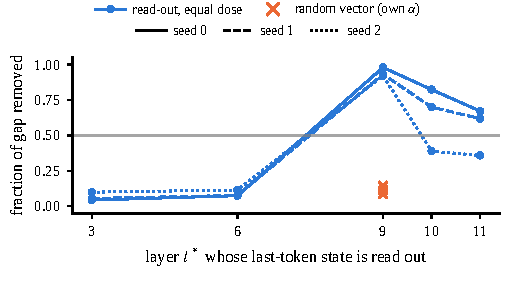
\includegraphics[width=\columnwidth]{figures/paper/fig_h_readout.pdf}
\caption{Read-out at equal total dose from layer $l^*$: fraction of the shortcut gap removed. Crosses: a random vector
with its own $\alpha$ under the same accuracy limit.}
\label{fig:readout}
\end{figure}

\textbf{What the fix is (post-hoc).} At the chosen strength the added signal dominates the last blocks, so the model
effectively answers from layer~9. Reading the answer directly from layer~9 with the calibrated lens gives nearly the same
result (Table~\ref{tab:readout}), and the two agree on \phAgreementFullFT{} of the test answers. We therefore present the
read-out as an early exit implemented inside the normal forward pass, not as a new steering method. What it adds to our
question is that its success depends on the location: the same dose from other layers works much less well.

\textbf{Caveats.} Layer~9 was identified from earlier analyses of the same models, so the read-out has not been tested
on a model where the layer was chosen blind; the equal-dose runs chose the largest $\alpha$ in their grid, so their
effects may be larger at higher doses; and in seed 1 the cue-free choice is close to the accuracy limit (drop
\pSixBCueFreeDropFullFTsOne).
